\chapter{Tolman-Oppenheimer-Volkoff equation}
\label{chap:tov}

In 1687, Sir Isaac Newton sparked a revolution in the field of physics when he described motion of bodies with the concept of forces and modeled gravity as an attractive force
\cite{ref:newton}
\begin{equation*}
	\vec{F} = G \frac{m_1 m_2}{r^2} \vec{\hat{r}} .
\end{equation*}
For a long time, his three laws of motion and law of gravity seemed to accurately explain all observable macroscopic motion.
In particular, his laws provided an explanation for the three laws of planetary motion that Johannes Kepler found by empirical observation many years earlier in 1609 \cite{ref:kepler1} and 1619 \cite{ref:kepler2}.

However, in 1859, Urbain Le Verrier observed that Mercury's orbit deviates from the one predicted by Kepler's and Newton's laws \cite{ref:le_verrier}.
The resolution came half a century later, when Albert Einstein proposed his theory of special relativity in 1905 \cite{ref:einstein_special} and ten years later incorporated gravity into this framework with the theory of general relativity \cite{ref:einstein_general}.
%Newton: gravity affects body, body does not move along straight path
%Einstein: gravity affects space, body moves along straight path
While Newton thought gravity \emph{disturbs a body} from moving straight through spacetime, Einstein explained gravity as \emph{curvature of spacetime} that instead reshapes the straight paths along which a body moves.
Such a ``curved straight path'' is called a \emph{geodesic}.
%While Newton thought gravity affects a body and disturbs its straight motion through flat space, Einstein instead thought gravity \emph{curves} space and thus changes the straight paths along which bodies move.
%Instead of describing gravity as a force that disturbs straight motion through flat space, Einstein argued that gravity rather \emph{curves} space and time and thus alters the paths along which straight motion occurs.
%Instead of describing gravity as a force that disturbs straight motion through flat space, Einstein explained that gravity \emph{curves} space and time and alters the paths along which straight motion occurs.
%Einstein argued that bodies \emph{do} move along straight paths through space and time that have been \emph{curved} by the presence of mass and energy according to the Einstein field equations
Spacetime is curved according to the Einstein field equations
\begin{equation*}
	G\indices{_\mu_\nu} = R_{\mu \nu} - \frac{1}{2} R g_{\mu \nu} = \frac{8 \pi G}{c^4} T_{\mu \nu} ,
\end{equation*}
expressing how energy and momentum on the rightmost side -- such as mass and light -- determine the geometry of spacetime on the left side.

The most important result of this chapter will be the Tolman-Oppenheimer-Volkoff equation
\begin{equation*}
	\odv{P(r)}{r} = -\frac{G m(r) \epsilon(r)}{r^2 c^2} \left[ 1 + \frac{P(r)}{\epsilon(r)} \right] \left[ 1 + \frac{4 \pi r^3 P(r)}{m(r) c^2} \right] \left[ 1 - \frac{2 G m(r)}{r c^2} \right]^{-1} ,
\end{equation*}
which we will derive from the Einstein field equations.
With this equation, we can find the pressure profile and radius of a star once we have an equation of state that relates the pressure and energy of the material inside.
This will be an essential tool for our following analysis of different equations of state.
The equation was originally derived in 1939 by Robert Oppenheimer and George Volkoff \cite{ref:tov}, building on earlier work of Richard Tolman \cite{ref:tolman}.

We will also examine the general consequences of this equation applied to the extreme case of an incompressible star. 
To make sense of our results, we will investigate the correspondence between general relativity and Newtonian gravity in the limit of small velocoties and weak gravitational fields.

\textit{This chapter is inspired by references \cite{ref:carroll}, \cite{ref:mtw} and \cite{ref:mika_gr_notes}.}

\section{Derivation from the Einstein field equations}
\label{sec:einstein_to_tov}

To analyze astrophysical objects like stars, it is of considerable interest to relate the pressure $P(x)$ and energy density $\epsilon(x)$ or mass density $\rho(x)$ at every position $x$ inside the object.
We will derive the relativistic relation between these quantities from the \textbf{Einstein field equations} \cite[equation 4.44]{ref:carroll}
\begin{equation}
	G\indices{_\mu_\nu} = R_{\mu \nu} - \frac{1}{2} R g_{\mu \nu} = \frac{8 \pi G}{c^4} T_{\mu \nu} .
	\label{eq:einstein}
\end{equation}
It describes how the geometry of spacetime, described by the Ricci tensor $R\indices{_\mu_\nu}$ and Ricci scalar $R$ that are ultimately built from the metric $g\indices{_\mu_\nu}$ and encapsulated in the Einstein tensor $G\indices{_\mu_\nu}$ (see \cref{chap:gr_summary} for a summary), responds to the presence of energy-momentum in the energy-momentum tensor $T\indices{_\mu_\nu}$.
Here, $G$ is the gravitational constant and $c$ is the speed of light.
As we later compare our findings to those of Newtonian gravity, it will be useful to connect the energy density to the mass density by the \textbf{mass-energy equivalence relation}
\begin{equation}
	\epsilon(x) = \rho(x) c^2 .
	\label{eq:tov:mass_energy_equivalence}
\end{equation}

Unless rotating very fast, stars are well approximated by spheres.
For our purposes, we therefore use the coordinates
\begin{equation}
	x^\mu = (c t, r, \theta, \phi)
	\quad \text{with} \quad
	-\infty < t < \infty, \quad
	0 \leq r < \infty, \quad
	0 \leq \theta \leq \pi, \quad
	0 \leq \phi < 2 \pi .
\end{equation}
and consider the most general line element that exhibits spherical symmetry, \cite[equation 5.11]{ref:carroll}
\begin{equation}
	% coordinates x = (ct, r, θ, ϕ)
	\dif s^2 = e^{2 \alpha(r)} c^2 \dif t^2 - e^{2 \beta(r)} \dif r^2 - r^2 \left( \dif \theta^2 + \sin^2 \theta \dif \phi^2 \right) .
\label{eq:tov:metric}
\end{equation}

We model the interior of the star as a perfect fluid with energy-momentum \cite[equation 1.114]{ref:carroll}
\begin{equation}
	T\indices{_\mu_\nu}(r) = \frac{U_\mu U_\nu}{c^2} \left[ \epsilon(r)+P(r) \right]  - g\indices{_\mu_\nu} P(r) .
	\label{eq:tov:energy_momentum_perfect_fluid}
\end{equation}
The analysis is simplest in the rest frame of the fluid, where $U_\mu = (U_0, \textbf{0})$ and the normalization condition $U_\mu U^\mu = c^2$ requires $U_0 = \pm e^\alpha c$.
We choose the positive sign so the four-velocity lies in the future light cone, as we are interested in the evolution of the star.
Dropping the function argument $r$ from now, the energy-momentum tensor then takes the diagonal form
\begin{equation}
T\indices{_\mu_\nu} =
\begin{bmatrix}
	\epsilon e^{2\alpha} & 0            & 0     & 0                   \\
	0                    & P e^{2\beta} & 0     & 0                   \\
	0                    & 0            & P r^2 & 0                   \\
	0                    & 0            & 0     & P r^2 \sin^2 \theta \\
\end{bmatrix}
\qquad \text{or} \qquad
T\indices{_\mu^\nu} =
\begin{bmatrix}
	\epsilon &  0 &  0 &  0 \\
	0        & -P &  0 &  0 \\
	0        &  0 & -P &  0 \\
	0        &  0 &  0 & -P \\
\end{bmatrix}
.
\label{eq:einstein_to_tov:T}
\end{equation}

Starting with the metric, it is now straightforward, although tedious, to compute the left side of \cref{eq:einstein} from \cref{eq:def_christoffel,eq:def_riemann_tensor,eq:def_ricci_tensor,eq:def_ricci_scalar}.
For the details, refer to \cite[equation 5.11-5.15]{ref:carroll} or \cref{sec:tov_cas_derivation}.
After inserting the energy-momentum tensor on the right and simplifying, we get the three independent equations
(the fourth turns out proportional to the third)
\begin{subequations}
\begin{align}
	\frac{1}{r^2} e^{-2 \beta} \left( 2 r \beta' - 1 + e^{2 \beta} \right)                               &= \frac{8 \pi G}{c^4} \epsilon
	&& \left( G\indices{_0_0} = \frac{8 \pi G}{c^4} T\indices{_0_0} \right) , \label{eq:einstein_to_tov:tt} \\
	\frac{1}{r^2} e^{-2 \beta} \left( 2 r \alpha' + 1 - e^{2 \beta} \right)                              &= \frac{8 \pi G}{c^4} P
	&& \left( G\indices{_1_1} = \frac{8 \pi G}{c^4} T\indices{_1_1} \right) , \label{eq:einstein_to_tov:rr} \\
	e^{-2 \beta} \left( \alpha'' + (\alpha')^2 - \alpha' \beta' + \frac{1}{r} (\alpha' - \beta') \right) &= \frac{8 \pi G}{c^4} P
	&& \left( G\indices{_2_2} = \frac{8 \pi G}{c^4} T\indices{_2_2} \right) . \label{eq:einstein_to_tov:thetatheta}
\end{align}
\label{eq:einstein_to_tov:einstein_equation_in_star}
\end{subequations}

Next, let us introduce the mass of the star.
Define the function $m(r)$ by
\begin{equation}
	e^{2 \beta(r)} = \left[ 1 - \frac{2 G m(r)}{r c^2} \right]^{-1} ,
	\label{eq:einstein_to_tov:def_m}
\end{equation}
so $g\indices{_1_1}$ resembles the Schwarzschild metric element.
Then \cref{eq:einstein_to_tov:tt} becomes
\begin{equation}
	\odv{\left[m(r) c^2\right]}{r} = 4 \pi r^2 \epsilon(r) ,
	\label{eq:einstein_to_tov:m_rho}
\end{equation}
directly relating $m(r)$ and $\epsilon(r)$.
If we set $m(0) = 0$, we can integrate to get
\begin{equation}
	m(r) c^2 = \integral{\epsilon(r') 4 \pi r'^2}{r'}{0}{r} .
	\label{eq:einstein_to_tov:m_integral}
\end{equation}
In \cite[page 602]{ref:mtw} it is shown that setting $m(0) \neq 0$ creates a singularity at the origin, which is not physically acceptable.
Outside a star that extends to $r = R$, there is vacuum with $\epsilon = 0$ and our metric should match the Schwarzschild metric with $g\indices{_1_1} = -(1-2GM/rc^2)^{-1}$ and Schwarzschild mass $M$ \cite[equation 5.1]{ref:carroll}.
By comparison with \cref{eq:einstein_to_tov:def_m}, the \textbf{Schwarzschild mass} of the star must be
\begin{equation}
	M = m(R) = \frac{1}{c^2} \integral{\epsilon(r) 4 \pi r^2}{r}{0}{R} = \integral{\rho(r) 4 \pi r^2}{r}{0}{R}.
	\label{eq:einstein_to_tov:schwarzschild_mass}
\end{equation}
It is tempting to interpret the Schwarzschild mass $M$ as the Newtonian mass of the star and \eqref{eq:einstein_to_tov:m_integral} as the volume integral of the energy density $\epsilon(r)$.
But $4 \pi r^2$ is not a proper volume element, as it does not involve the full spatial metric determinant.
We return to this question in \cref{sec:weak_field_limit} after studying incompressible stars in \cref{sec:incompressible_star}, where we will see that the first interpretation is correct, while the latter is more subtle and differs by the binding energy of the star.

Meanwhile, definition \eqref{eq:einstein_to_tov:def_m} turns \cref{eq:einstein_to_tov:rr} into
\begin{equation}
	\odv{\alpha(r)}{r} = \frac{G}{r^2 c^4} \frac{m(r) c^2 + 4 \pi r^3 P(r)}{1 - 2 G m(r) / r c^2} .
	\label{eq:einstein_to_tov:dadr1}
\end{equation}
To finally eliminate $\alpha$, we can replace all occurences of $\alpha'$ and $\beta$ in the remaining \cref{eq:einstein_to_tov:thetatheta} with the expressions \eqref{eq:einstein_to_tov:dadr1} and \eqref{eq:einstein_to_tov:def_m}.
Doing so is straightforward, but cumbersome and most easily done by a computer algebra system.
We show how to do this in \cref{sec:tov_cas_derivation}.
An elegant, but less straightforward argument is to use local energy-momentum conservation $\nabla_\mu T\indices{^\mu^\nu} = 0$, which is both physically reasonable and in fact possible to prove directly from the Einstein field equations \eqref{eq:einstein}.
For two different proofs, see \cite{ref:einstein_conservation_energy_momentum} and \cite[section 8.3.2]{ref:mika_gr_notes}.
Using \cref{eq:def_cov_deriv}, the component $\nu=1$ gives
\begin{equation*}
	0
	= \nabla_\mu T\indices{^\mu_1}
	= \partial_1 T\indices{^1_1} + \Gamma^\sigma_{1 \sigma} T\indices{^1_1} - \Gamma^\sigma_{1 \mu} T\indices{^\mu_\sigma}
	= \partial_1 T\indices{^1_1} + \Gamma^0_{10} T\indices{^1_1} + \sum_{i=1}^3 \Gamma^i_{1i} T\indices{^1_1} - \Gamma^0_{10} T\indices{^0_0} - \sum_{i=1}^3 \Gamma^i_{1i} T\indices{^i_i}
\end{equation*}
Using $T\indices{^0_0} = \epsilon$ and $T\indices{^1_1} = T\indices{^2_2} = T\indices{^3_3} = -P$ from \cref{eq:einstein_to_tov:T}, the explicit sums cancel.
With $\Gamma^0_{10} = \frac12 g^{00} \partial_1 g_{00} = \odv{\alpha}/{r}$, we are left with
\begin{equation}
	\odv{\alpha}{r} = \frac{-1}{\epsilon+P} \odv{P}{r} .
	\label{eq:einstein_to_tov:dadr2}
\end{equation}
Now $\alpha$ is easily eliminated by equating \eqref{eq:einstein_to_tov:dadr1} and \eqref{eq:einstein_to_tov:dadr2}. 
Whichever approach we follow, we end up with the \textbf{Tolman-Oppenheimer-Volkow (TOV) equation}
\begin{equation}
	\odv{P(r)}{r} = -\frac{G m(r) \epsilon(r)}{r^2 c^2} \left[ 1 + \frac{P(r)}{\epsilon(r)} \right] \left[ 1 + \frac{4 \pi r^3 P(r)}{m(r) c^2} \right] \left[ 1 - \frac{2 G m(r)}{r c^2} \right]^{-1} .
	\label{eq:tov}
\end{equation}
It relates the pressure gradient $\odv{P}/{r}$ and energy density $\epsilon$ at radius $r$ from the center of a spherical static star composed of a perfect fluid.
\Cref{eq:einstein_to_tov:m_rho,eq:tov} constitute two equations for the three unknowns $P$, $\epsilon$ and $m$.
To determine them, an additional \textbf{equation of state}
\begin{equation}
	F(P, \epsilon) = 0
\label{eq:tov:eos}
\end{equation}
that relates the thermodynamic variables is required, typically obtained from statistical physics.
Given all three equations and the central pressure $P(0)$, we can integrate to find the pressure everywhere inside the star.
We define the radius of the star to be the radius $R$ at which $P(R) = 0$.
Carrying out this procedure for different values of $P(0)$, we can find a mass-radius relation $M(R)$ for stars parametrized by their central pressure $P(0)$.

\section{Solution for an incompressible star}
\label{sec:incompressible_star}

% TODO: an incompressible star is unphysical

Although it may sound unphysical from the outset, we can make a somewhat realistic model of a star by assuming that the fluid is incompressible, meaning the energy density
\begin{equation}
	\epsilon(r) = \epsilon_0
\end{equation}
is constant inside the star.
For example, this results in a completely unrealistic speed of sound $v = \sqrt{\odv{P}/{\rho}} = c \sqrt{1/(\odv{\epsilon}/{P})} = c \sqrt{1/0} = \infty$ \cite{ref:speed_of_sound}.
Anyway, integrating \cref{eq:einstein_to_tov:m_integral,eq:einstein_to_tov:schwarzschild_mass} yield
\begin{equation}
	m(r) c^2 = \frac{4}{3} \pi r^3 \epsilon_0 
	\quad \text{and} \quad
	M c^2 = \frac{4}{3} \pi R^3 \epsilon_0 
	.
\end{equation}
Inserting the energy density $\epsilon(r)$ and mass $m(r)$ into \cref{eq:tov}, $P$ and $r$ separate to
\begin{equation*}
	\int \frac{\dif P}{(\epsilon_0+P)(\epsilon_0+3P)} = - \int \frac{4 \pi G r \dif r}{3 c^4 - 8\pi G r^2 \epsilon_0} .
\end{equation*}
The left side can now be split by the partial fraction decomposition
\begin{equation*}
	\frac{1}{(\epsilon_0+P)(\epsilon_0+3P)} = \frac{1}{2P} \left( \frac{1}{\epsilon_0+P} + \frac{1}{\epsilon_0+3P} \right) .
\end{equation*}
Performing all three integrals using the general antiderivatives
\begin{equation*}
	\int \frac{\dif x}{a x^2 + b x} = -\frac{1}{b} \log \left( a + \frac{b}{x} \right) + C
	\quad \text{and} \quad
	\int \frac{x \dif x}{a x^2 + b} = \frac{1}{2 a} \log \left( a x^2 + b \right) + C
\end{equation*}
and applying the boundary condition $P(R) = 0$ to determine the integration constant, we eventually find the radial pressure
\begin{equation}
	% p(r) in terms of M, R, 
	P(r) = \epsilon_0 \, \frac{\sqrt{1-\frac{2GMr^2}{R^3c^2}} - \sqrt{1-\frac{2GM}{Rc^2}}}{3 \sqrt{1-\frac{2GM}{Rc^2}} - \sqrt{1-\frac{2GMr^2}{R^3c^2}}} .
	% p(r) in terms of p0, M, R
	%p(r) = -\frac{M}{\frac{4}{3} \pi R^3} \frac{4 \pi R^{3} p_0 \left( \frac{1}{3} + \sqrt{1-\frac{2GMr^2}{R^3}} \right) + M \left( 1 + \sqrt{1-\frac{2GMr^2}{R^3}} \right)}
	%                                           {4 \pi R^{3} p_0 \left( 1           + \sqrt{1-\frac{2GMr^2}{R^3}} \right) + M \left( 3 + \sqrt{1-\frac{2GMr^2}{R^3}} \right)}
	\label{eq:incompressible_star:pressure}
\end{equation}
In particular, the central pressure is
\begin{equation}
	P(0) = \epsilon_0 \frac{1 - \sqrt{1 - \frac{2GM}{Rc^2}}}{3 \sqrt{1-\frac{2GM}{Rc^2}} - 1} .
	\label{eq:incompressible_star:central_pressure}
\end{equation}
It is interesting to note that the pressure is positive for $GM/Rc^2 < 4/9$, but explodes at $GM/Rc^2 = 4/9$ and becomes negative for $GM/Rc^2 > 4/9$.
The pressure profile of stars approaching this limit is shown in \cref{fig:incompressible_star:plot2}.
Physically, this means that any star compressed to this limit could only be supported by an unattainable infinite central pressure, so it would have no other choice than to collapse.
This is an example of a more general result -- \textbf{Buchdal's theorem} states that all static spherical stars composed of perfect fluids must have
\begin{equation}
	M(R) < M_\text{max}(R) = \frac{4c^2}{9G} R
	\label{eq:incompressible_star:buchdal}
\end{equation}
for any energy density profile $\epsilon(r)$ that does not decrease outwards \cite{ref:buchdal}.
The proof requires careful work, but we can still understand the result intuitively.
If there is a maximum density that is supported by nature, then the most massive object we can make would necessarily have that density everywhere.
Thus, the bound we have found in our computation with constant energy density should be the most extreme bound.
In \cref{fig:incompressible_star:plot1}, we compare the mass-radius relation to this maximum supported mass.

% Ideal use of groupplot + subcaption:
% * use title={\subcaption{...}} for subcaptions (https://tex.stackexchange.com/a/310403)
% * set title style text width automatically (https://tex.stackexchange.com/a/276214)
% * another example (https://tex.stackexchange.com/a/69729)
\begin{figure}[ht!]
	\centering
	\begin{tikzpicture}[declare function={
		G = 1;
		M(\R,\E) = 4/3*pi*(\R)^3*\E;
		Mmax(\R) = 4*\R/(9*G);
		p(\r,\M,\R) = \M / (4/3*pi*(\R)^3) * (sqrt(1-2*G*\M*(\r)^2/(\R)^3) - sqrt(1-2*G*\M/(\R))) / (3*sqrt(1-2*G*\M/(\R)) - sqrt(1-2*G*\M*(\r)^2/(\R)^3));
	}]
		\begin{groupplot}[group style={group size=2 by 1, horizontal sep=0.1\textwidth}, width=0.49\textwidth]
		\nextgroupplot[
			title={\subcaption{\label{fig:incompressible_star:plot1}Mass-radius relation}},
			xlabel=$R \, / \, R_0$, ylabel=$M(R) \, / \, M(R_0)$, xtick distance=1, 
			legend pos=north west, legend cell align=left,
		]
		\pgfplotsinvokeforeach{0.006} {
			\addplot [domain=0:5, solid ] {M(x,#1) / M(1,#1)}; % node[pos=0.90, sloped, yshift=+6pt] {\scriptsize $\epsilon_0 = #1$};
			\addplot [domain=0:5, dashed] {Mmax(x) / M(1,#1)}; % node[pos=0.2, pin=above:{$M_\text{max}(R)$}] {};
		}
		\legend{$M(R)$, $M_\text{max}(R)$};
		\nextgroupplot[
			title={\subcaption{\label{fig:incompressible_star:plot2}Pressure profile}},
			xlabel=$r\, /\, R_0$, ylabel=$P(r) \, / \, P(0)$, xtick distance=0.25,
		]
		\pgfplotsinvokeforeach{0.9, 0.99, 0.999} {
			\addplot [domain=0:1,samples=200] {p(x,#1*Mmax(1),1)/p(0,#1*Mmax(1),1)} node[pos=0.54, sloped, yshift=+16pt] {\scriptsize $M = #1 M_\text{max}$};
		}
		\end{groupplot}
	\end{tikzpicture}
	\caption{
		\subref{fig:incompressible_star:plot1} Mass-radius relation $M(R) = 4 \pi R^3 \epsilon_0 / 3 c^2$ for a star of constant energy density $\epsilon_0$ compared to the maximum supported mass $M_\text{max}(R) = 4 c^2 R / 9 G$.
		\subref{fig:incompressible_star:plot2} Pressure profile $P(r)$ for stars of radius $R_0 = \sqrt{c^4 / G \epsilon_0}$ and masses $M$ approaching the limit $M_\text{max}(R_0)$.
	}
\end{figure}

Another way of looking at the Buchdal's theorem is that the radius of a star must satisfy
\begin{equation}
	R > \frac94 \frac{G M}{c^2} = \frac98 R_S ,
\end{equation}
where $R_S = 2 G M / c^2$ is the \textbf{Schwarzschild radius} of the star.
In general relativity, it is a well known result of the spherical Schwarzschild solution that anything that falls into $r < R_S$ outside a massive body $M$ can never escape back out to $r > R_S$ \cite[section 5.6]{ref:carroll}.
Such a one-way gate is called an event horizon, and any object whose physical radius is smaller than its Schwarzschild radius is called a \textbf{black hole}.
Not even light can escape from a black hole, so it is completely invisible for outside observers -- hence the name.
Thus, a stable star that satisfies the Buchdal bound $R > 9 G M / 4 c^2$ is not a black hole.
If we somehow \emph{do} manage to compress a star to the radius $R = 9 G M / 4 c^2$, it would be unsustainable, implode and turn into a black hole.

In \cref{sec:weak_field_limit} we will see that Buchdal's theorem is a relativistic result and that no such bound arises from Newtonian gravity.

\section{Newtonian limit and physical interpretation of mass}
\label{sec:weak_field_limit}

%TODO: move everything about interpretation of mass, energy density integral etc. to one section which has one thing in common: we look at the weak-field limit
%TODO: do weak-field limit of TOV equation, too

In Newtonian gravity, the presence of mass $\rho(\vec{x})$ produces a gravitational field $-\nabla V(\vec{x})$ through the Poisson equation
\begin{equation}
	\nabla^2 V(\vec{x}) = 4 \pi G \rho(\vec{x}) .
	\label{eq:interpretation_m:poisson}
\end{equation}
In turn, matter respond to the field as particles are accelerated by
\begin{equation}
	\odv[2]{\vec{x}}{t} = - \nabla V(\vec{x}) .
	\label{eq:interpretation_m:newton2}
\end{equation}
Given the initial distribution and velocities of matter, these two coupled differential equations determine its movement forever and thus contain all of Newtonian gravity.
Here we will show that general relativity is reducible to Newtonian gravity in the \textbf{Newtonian limit} characterized by \emph{slow movement} and a \emph{static} and \emph{weak} gravitational field.
In particular, we will demonstrate that the response of matter to the field \eqref{eq:interpretation_m:newton2} follows from the geodesic equation \eqref{eq:geodesic}, and similarly that the response of the field to matter \eqref{eq:interpretation_m:poisson} follows from the Einstein field equations \eqref{eq:einstein}.
Having established this correspondence, we move on to interpret the ``mass'' $M$ and ``energy'' $Mc^2$ that we encountered in \cref{eq:einstein_to_tov:schwarzschild_mass}, but struggled to understand the meaning of.
Finally, we derive the Newtonian pressure gradient analogous to the relativistic gradient \eqref{eq:tov} and show that the latter reduces to the former in the Newtonian limit.

Before we set out, however, let us make the Newtonian limit mathematically precise.
First, by \emph{slow movement}, we mean that all velocities $v$ are much lower than the speed of light $c$, so
\begin{subequations}
\begin{equation}
	\frac{v}{c} \ll 1 .
	\label{eq:weak_field_limit:small_velocity}
\end{equation}
In a potential $V$ measured with respect to $V(\infty) = 0$, freely falling particles are accelerated to kinetic energies on the scale $\frac12 m v^2 = m V$.
Consequently, particles could reach velocities that violate criterion \eqref{eq:weak_field_limit:small_velocity} unless the potential is bounded by
\begin{equation}
	\frac{V}{c^2} \ll 1 .
	\label{eq:weak_field_limit:small_potential}
\end{equation}
In the presence of a fluid with energy-momentum \eqref{eq:tov:energy_momentum_perfect_fluid}, internal stresses in the fluid also generate motion.
For example, the energy-momentum \eqref{eq:einstein_to_tov:T} would give rise to sound waves propagagating with velocity $v = \sqrt{\odv{P}/{\rho}} = c \sqrt{-\odv{T\indices{_i^i}}/{T\indices{_0^0}}}$, with no sum over $i$.
More generally, we therefore assume slow movement corresponds to $\odv{T_{ij}}/{T_{00}} \ll 1$ or, by integration,
\begin{equation}
	\frac{T_{ij}}{T_{00}} \ll 1 .
	\label{eq:weak_field_limit:small_pressure}
\end{equation}
\end{subequations}
Glancing back at \cref{eq:tov:energy_momentum_perfect_fluid}, we see that we can neglect pressure $P$ in favor of energy density $\epsilon$ in the Newtonian limit.
This result can be understood physically -- pressure is a result of randomized motion and decreases with the velocities of the motion, while energy is equivalent to mass and is unaffected by the velocity of the mass.
In summary, slow motion is achieved only if \cref{eq:weak_field_limit:small_velocity,eq:weak_field_limit:small_potential,eq:weak_field_limit:small_pressure} are all satisfied.

Second, the assumption of a \emph{static} gravitational field means that all time derivatives of the metric vanish like
\begin{equation}
	\partial_0 g_{\mu \nu} = 0 .
	\label{eq:weak_field_limit:static_field}
\end{equation}

Third, a \emph{weak} field corresponds to a metric that can be written as a perturbation
\begin{equation}
	g\indices{_\mu_\nu} = \eta\indices{_\mu_\nu} + h\indices{_\mu_\nu}
	\qquad \text{with} \qquad
	\abs{h\indices{^\mu^\nu}} \ll 1
	\label{eq:weak_field_limit:weak_field_metric}
\end{equation}
on top of flat Minkowski space $\eta\indices{^\mu^\nu} = \text{diag}(+1, -1, -1, -1)$.
The inverse metric $g\indices{^\mu^\nu}$ should satisfy $g\indices{^\mu^\nu} g\indices{_\nu_\sigma} = \delta^\mu_\sigma$, so to first order in $h$ we must have
\begin{equation}
	g\indices{^\mu^\nu} = \eta\indices{^\mu^\nu} - h\indices{^\mu^\nu} ,
	\label{eq:weak_field_limit:weak_field_metric_inverse}
\end{equation}
where $h\indices{^\mu^\nu} = \eta\indices{^\mu^\rho} \eta\indices{^\nu^\sigma} h\indices{_\rho_\sigma}$ is raised with the \emph{Minkowski} metric.

\subsection{Newtonian limit of the response of matter to the field}

In general relativity, matter responds to the gravitational field by moving along geodesics $x(\tau)$ that satisfy the \textbf{geodesic equation}
\begin{equation}
	\odv[2]{x^\mu}{\tau} + \Gamma^\mu_{\rho \sigma} \odv{x^\rho}{\tau} \odv{x^\sigma}{\tau} = 0 .
	\label{eq:geodesic_duplicate}
\end{equation}
We explain the origin of the geodesic equation in \cref{sec:geodesic}, where we show that moving along geodesics corresponds to taking the shortest possible path between points in spacetime.
Let us now show that we recover the Newtonian response \eqref{eq:interpretation_m:newton2} in the Newtonian limit.

The criterion of slow movement \cref{eq:weak_field_limit:small_velocity} implies that a particle with velocity $\odv{x^\mu}/{\tau}$ has spatial components $\odv{x^i}/{t} \ll c$ and must be dominated by the temporal component $c \odv{t}/{\tau} \approx c$.
Then $\odv{x^i}/{\tau} \ll \odv{x^0}/{\tau}$ and the geodesic equation can be approximated by
\begin{equation}
	\odv[2]{x^\mu}{\tau} + \Gamma^\mu_{00} \, c^2 \left( \odv{t}{\tau} \right)^2 = 0 .
	\label{eq:weak_field_limit:geodesic_approximated}
\end{equation}
In a static field, the vanishing time derivatives \eqref{eq:weak_field_limit:static_field} simplifies the Christoffel symbols \eqref{eq:def_christoffel} to $\Gamma^\mu_{00} = -\frac{1}{2} g\indices{^\mu^\lambda} \partial_\lambda g\indices{_0_0}$.
Inserting the weak-field metric \eqref{eq:weak_field_limit:weak_field_metric} and its inverse \eqref{eq:weak_field_limit:weak_field_metric_inverse} and calculating to first order in $h$, we find the Christoffel symbols
\begin{equation}
	\Gamma^\mu_{00} = -\frac{1}{2} \eta\indices{^\mu^\lambda} \partial_\lambda h\indices{_0_0} .
	\label{eq:weak_field_limit:static_christoffel_symbols}
\end{equation}
In particular, the static metric implies that $\Gamma^0_{00} = 0$, so $\odv[2]{t}/{\tau} = 0$ by the approximated geodesic equation \eqref{eq:weak_field_limit:geodesic_approximated}.
As we have neglected $\odv{x^i}/{\tau}$, we can now regard $x(\tau) = x(\tau(t))$ as a function of only $t$ and apply the chain rule and the product rule to get 
\begin{equation}
	\odv[2]{x}{\tau} = \odv*{\left( \odv{x}{t} \odv{t}{\tau} \right)}{\tau} = \left( \odv[2]{x}{t} \right) \left( \odv{t}{\tau} \right)^2 + \left( \odv{x}{t} \right) \left( \odv[2]{t}{\tau} \right) = \left( \odv[2]{x}{t} \right) \left( \odv{t}{\tau} \right)^2 .
\end{equation}
Upon insertion into the \cref{eq:weak_field_limit:geodesic_approximated}, we can cancel the common factor $(\odv{t}/{\tau})^2$ and write the geodesic equation purely in terms of time $t$ as
\begin{equation*}
	\odv[2]{x^\mu}{t} = \frac{1}{2} c^2 \eta\indices{^\mu^\lambda} \partial_\lambda h\indices{_0_0} .
\end{equation*}
The spatial components of this equation is precisely Newton's second law \cref{eq:interpretation_m:newton2} if we identify $h\indices{_0_0} = 2V/c^2$.
In conclusion, we have showed that a weak relativistic gravitational field with
\begin{equation}
	g\indices{_0_0} = 1 + h_{00} = 1 + \frac{2V}{c^2} 
	\label{eq:weak_field_limit:metric_with_potential}
\end{equation}
describes Newtonian motion in the gravitational potential $V$!

\subsection{Newtonian limit of the response of the field to matter}
\label{sec:einstein_to_poisson}

In general relativity, the gravitational field is produced by matter that enter the Einstein field equations \eqref{eq:einstein} on the right.
Let us show that they fall back the Poisson equation \eqref{eq:interpretation_m:poisson} to first nonzero order in the metric perturbation $h$ of the Newtonian limit.

Suppose we are in the stationary reference frame of a perfect fluid with energy-momentum \eqref{eq:tov:energy_momentum_perfect_fluid} and velocity $U^\mu = (U^0, \vec{0})$.
To first order in $h_{00}$, the normalization condition $U^\mu U_\mu = c^2$ then fixes the time component
\begin{equation}
	U^0 = \frac{c}{\sqrt{g_{00}}} = \frac{c}{\sqrt{1 + h_{00}}} \taylor c \left( 1 - \frac12 h_{00} \right) .
\end{equation}
To lowest order, the energy-momentum \eqref{eq:tov:energy_momentum_perfect_fluid} then simplifies to dust with
\begin{equation}
	T_{00} = \rho U_0 U_0 \taylor \epsilon
	\qquad \text{and trace} \qquad
	T = T\indices{^\mu_\mu} = g^{00} T_{00} \taylor \epsilon, 
\end{equation}
and the pressure components are negligible according to \cref{eq:weak_field_limit:small_pressure}.
Now rewrite the Einstein field equations \eqref{eq:einstein} by taking the trace of both sides.
Using $g\indices{^\mu_\mu} = \delta\indices{^\mu_\mu} = 4$, we find that the Ricci scalar can be expressed as $R = - 8 \pi G T / c^4$, so the field equations are equivalent to
\begin{equation}
	R_{\mu \nu} = \frac{8 \pi G}{c^4} \left( T_{\mu \nu} - \frac12 T g_{\mu \nu} \right) .
	\label{eq:einstein_rewritten}
\end{equation}
Inserting our results from above, we find the Ricci tensor element
\begin{equation}
	R_{00} = \frac{4 \pi G \rho}{c^2} .
	\label{eq:weak_field_limit:ricci_from_energy_momentum}
\end{equation}

Instead of calculating the Ricci tensor from the energy-momentum of matter, we can attack the problem from the geometric point of view and find it from the Riemann curvature tensor
\begin{equation}
	R\indices{^\rho_0_\mu_0} =
	\partial\indices{_\mu} \Gamma^\rho_{0 0} -
	\partial\indices{_0} \Gamma^{\rho}_{\mu 0} +
	\Gamma^\rho_{\mu \lambda} \Gamma^{\lambda}_{0 0} -
	\Gamma^\rho_{0 \lambda} \Gamma^{\lambda}_{\mu 0} .
\end{equation}
Each Christoffel symbol is of order $\bigo(h)$, so all the products are all of order $\bigo(h^2)$.
Additionally, the time derivative vanishes for our stationary metric, so we are left with only $R\indices{^\rho_0_\mu_0} = \partial_\mu \Gamma^\rho_{00}$ to first order.
Using the stationary Christoffel symbols \eqref{eq:weak_field_limit:static_christoffel_symbols}, the Ricci tensor is
\begin{equation}
	R_{00} =       R\indices{^\mu_{0 \mu 0}}
		   %=       -\frac12 g^{\mu \nu} \partial_\mu \partial_\nu g_{00}
		   %=       -\frac12 g^{i j} \partial_i \partial_j g_{00}
		   = \partial_\mu \Gamma^\mu_{00}
		   = -\frac12 \eta^{\mu \lambda} \partial_\mu \partial_\lambda h_{00}
		   \taylor  \frac12 \delta^{i j} \partial_i \partial_j h_{00}
		   =        \frac12 \nabla^2 h_{00} .
	\label{eq:weak_field_limit:ricci_from_riemann}
\end{equation}

Inserting $h_{00} = 2V/c^2$ from \cref{eq:weak_field_limit:metric_with_potential} and comparing the result to \cref{eq:weak_field_limit:ricci_from_energy_momentum}, we see that the Einstein field equations yield the Poisson equation \eqref{eq:interpretation_m:poisson} in the Newtonian limit!

\subsection{Interpretation of mass and integrated energy density}

When we introduced the Schwarzschild mass $M$ given by \cref{eq:einstein_to_tov:schwarzschild_mass} in \cref{sec:einstein_to_tov}, we did not find it obvious how to interpret it.
Outside a star, spacetime is described by the Schwarzschild metric with the element \cite[equation 5.1]{ref:carroll}
\begin{equation}
	g\indices{_0_0} = 1 - \frac{2 G M}{r c^2}
	\quad \text{with} \quad
	h\indices{_0_0} = -\frac{2GM}{rc^2} .
	\label{eq:weak_field_limit:schwarzschild_metric_tt}
\end{equation}
But $V = c^2 h\indices{_0_0} / 2 = -G M / r$ is precisely the solution to the Poisson equation \eqref{eq:interpretation_m:poisson} for a spherical mass distribution, so we can in fact interpret the mass $M$ as the Newtonian mass of the star.
This is reassuring, as it allows us to measure masses of distant stars using Newtonian results like Kepler's third law \cite[chapter 19]{ref:mtw} that rely only on observations.

From the looks of \cref{eq:einstein_to_tov:schwarzschild_mass}, it is very tempting to also interpret $M c^2$ as the volume integral of the energy density over the star and thus its total energy.
But $4 \pi r^2 \dif r$ is not a proper volume element.
In a proper spatial integral, the volume element should be $\sqrt{\det{\gamma}} \dif^3 x = e^\beta r^2 \sin \theta \dif r \dif \theta \dif \phi$, where $\gamma\indices{_i_j} = g\indices{_i_j}$ is the spatial part of the metric and $\det{\gamma}$ its determinant.
So the true volume integral of the energy density is really
\begin{equation*}
	\bar{M} c^2 = \integral{\epsilon(r) e^{\beta(r)} 4 \pi r^2}{r}{0}{R} .
\end{equation*}
The difference
\begin{equation*}
	\bar{M} c^2 - M c^2 = \integral{\epsilon(r) \left[ \left( 1-\frac{2Gm(r)}{rc^2} \right)^{-1/2} - 1 \right] 4 \pi r^2}{r}{0}{R} > 0
\end{equation*}
is in fact the binding energy that arises due to the gravitational attraction between the individual fluid elements in the star.
To see this, consider again the weak-field limit.
Comparing \cref{eq:weak_field_limit:weak_field_metric,eq:weak_field_limit:schwarzschild_metric_tt}, we see that we have the small parameter
\begin{equation}
	\frac{G m(r)}{rc^2} \ll 1 .
	\label{eq:weak_field_limit:small_gmr}
\end{equation}
Using the Taylor expansion $(1 - x)^{-1/2} = 1 + x/2$ and the mass-energy equivalence relation \eqref{eq:tov:mass_energy_equivalence}, we get
\begin{equation}
	\bar{M} c^2 - M c^2 \taylor \integral{\frac{\epsilon(r)}{c^2} \frac{GM}{r} 4 \pi r^2}{r}{0}{R}
	                    =       \integral{\rho(r) \frac{GM}{r} 4 \pi r^2}{r}{0}{R} .
\end{equation}
As shown in \cite[exercise 23.7]{ref:mtw}, this is precisely the energy required to construct the star by sequentially placing thin shells of mass $\dif m = \rho(r) 4 \pi r^2 \dif r$ on top of each other, each subject to the gravitational attraction of the shells already placed below it.
This explains that $\bar{M} c^2 - M c^2$ is indeed the binding energy that would be required to disperse all the matter in the star to infinity.
Although we saw it was correct to interpret $M$ as the Newtonian mass of the star, it is \emph{not} correct to interpret $Mc^2$ as its total energy.
% confusion about M, \bar{M}, resources:
% https://physics.stackexchange.com/q/196280/299916
% see MTW p. 602-, box at p. 603, p. 453
% see Schwarz p. 126

\subsection{Newtonian limit of the TOV equation}

Finally, let us compare the TOV equation \eqref{eq:tov} and findings for relativistic incompressible stars from \cref{sec:incompressible_star} to those of Newtonian gravity.
To do so, we should first establish the Newtonian pressure gradient analogous to the relativistic one.

\begin{figure}
\centering
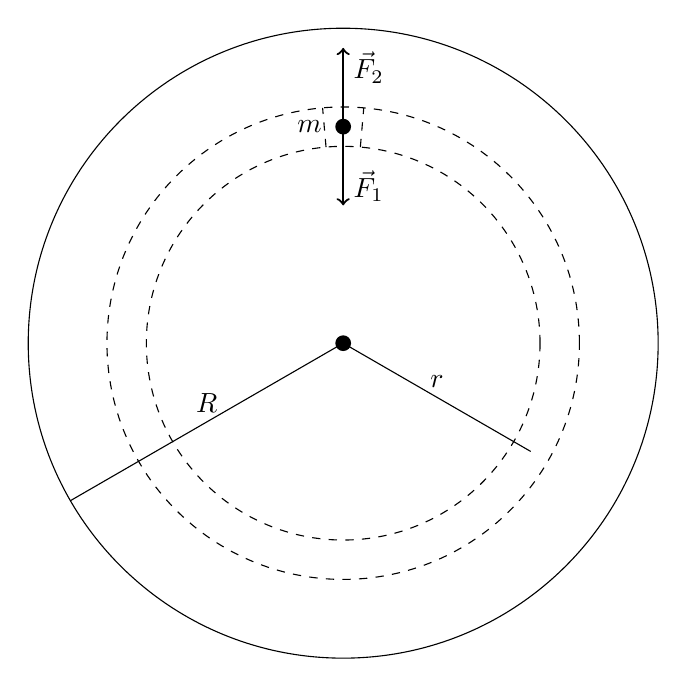
\begin{tikzpicture}
\draw[dashed] (85:2.5) -- (85:3.0);
\draw[dashed] (95:2.5) -- (95:3.0);
\draw [->, thick] (90:2.75) -- (90:1.75) node [near end, right] {$\dif \vec{F}_1$};
\draw [->, thick] (90:2.75) -- (90:3.75) node [near end, right] {$\dif \vec{F}_2$};
\fill (90:2.75) circle [radius=0.1cm];
\node[left=0.15cm] at (90:2.75) {$\dif m$};
\draw[dashed] (0,0) circle [radius=3cm];
\draw[dashed] (0,0) circle [radius=2.5cm];
\draw (0,0) circle [radius=4.0cm];
\fill (0,0) circle [radius=0.1cm];
\draw (0,0) -- (-30:2.75) node [midway,above] {$r$};
\draw (0,0) -- (210:4.0) node [midway,above] {$R$};
\end{tikzpicture}
\caption{\label{fig:hydrostatic_equilibrium_sphere}When a star of radius $R$ is in hydrostatic equilibrium, the gravitational force $\dif \vec{F}_1$ acting on a mass element  $\dif m$ at distance $r$ from the center must exactly cancel the pressure gradient force $\dif \vec{F}_2$.}
\end{figure}

Following \cref{fig:hydrostatic_equilibrium_sphere}, consider the mass element $\dif m = \rho(r) \dif A \dif r$ at distance $r$ from the center of a Newtonian star.
By Gauss' law it is attracted to the mass $m(r)$ inside the radius $r$ as if it were concentrated at the center, but experiences no attraction whatsoever from the remaining mass outside $r$ due to symmetry.
By Newton's law of gravity it is therefore pulled upon by the force
\begin{equation}
	\dif \mathbf{F}_1 = -\frac{G m(r) \dif m}{r^2} \hat{\textbf{r}} .
	\label{eq:weak_field_limit:force_newton}
\end{equation}
If the star is in hydrostatic equilibrium, this force must be exactly cancelled by the force
\begin{equation}
	\dif \textbf{F}_2 = - \Big[ P(r + \dif r) - P(r) \Big] \dif A \, \hat{\textbf{r}} = -\dif P \dif A \, \hat{\textbf{r}}
	\label{eq:weak_field_limit:force_pressure}
\end{equation}
that arises from the pressure difference above and below the element.
Setting $\dif \textbf{F}_1 + \dif \textbf{F}_2 = 0$ then gives the \textbf{Newtonian pressure gradient}
\begin{equation}
	\odv{P}{r} = -\frac{G m(r) \rho(r)}{r^2} .
	\label{eq:weak_field_limit:newtonian_pressure_gradient}
\end{equation}

Solving this differential equation for a star of constant mass density $\rho(r) = \rho_0$ like we solved the TOV equation \eqref{eq:tov} in \cref{sec:incompressible_star}, we get the pressures
\begin{equation}
	P(r) = \frac{\rho_0}{2} \frac{G M}{R} \left( 1 + \frac{r}{R} \right) \left( 1 - \frac{r}{R} \right)
	\quad \text{and} \quad
	P(0) = \frac{\rho_0}{2} \frac{GM}{R} .
	\label{eq:weak_field_limit:newtonian_pressure}
\end{equation}
In this case, the pressure is well-behaved for all $r$.
This shows that Buchdal's theorem \eqref{eq:incompressible_star:buchdal} is a purely \emph{relativistic} result, and that no such limitation arises in Newtonian gravity!

% TODO: makes us suspect that Newton is taylor expansion of TOV
% TODO: check limit

We expect that the Newtonian gradient \eqref{eq:weak_field_limit:newtonian_pressure_gradient} follows from the relativistic gradient \eqref{eq:tov} in the Newtonian limit.
Comparing the two, we see that the latter indeed reduces to the former \emph{if} all the corrections to $1$ in the three parentheses vanish.
This should come as no surprise, as we already saw in \cref{sec:einstein_to_poisson} that we recover Newtonian gravity from general relativity in this limit.
For example, the pressure \eqref{eq:weak_field_limit:newtonian_pressure} is precisely what one finds by Taylor expanding the relativistic pressure \eqref{eq:incompressible_star:pressure} about the small parameter \eqref{eq:weak_field_limit:small_gmr}.
To see that everything is consistent, let us nevertheless verify explicitly that this is the case.

First, note that the quantity \eqref{eq:weak_field_limit:small_gmr} in the rightmost parenthesis can be neglected.
Second, by \cref{eq:weak_field_limit:small_pressure}, we can neglect the pressure-energy density ratio
\begin{equation}
	\frac{P}{\epsilon} \ll 1
	\label{eq:weak_field_limit:small1}
\end{equation}
in the leftmost parenthesis.
Third, we argued in \cref{sec:incompressible_star} that all physical stars have non-increasing energy density $\epsilon(r)$ away from the center $r=0$.
We can then pull the minimum density $\epsilon(r)$ outside the integral \eqref{eq:einstein_to_tov:m_integral} to bound $m(r) c^2 \geq \frac{4}{3} \pi r^3 \epsilon(r)$.
It follows from \cref{eq:weak_field_limit:small1} that
\begin{equation}
	\frac{4 \pi r^3 P(r)}{m(r) c^2} \leq \frac{4 \pi r^3 P(r)}{\frac{4}{3} \pi r^3 \epsilon(r)}
	                                =    \frac{3 P(r)}{\epsilon(r)}
						            \ll  1 .
	\label{eq:weak_field_limit:small2}
\end{equation}
Thus, all three corrections in \cref{eq:tov} vanish, so we do indeed recover the Newtonian pressure gradient from the relativistic one in the Newtonian limit!

In fact, there is an alternative way to see it that requires much less work.
Replacing energy density $\epsilon$ with mass density $\rho$ using \cref{eq:tov:mass_energy_equivalence}, \cref{eq:tov} takes the form
\begin{equation}
	\odv{P(r)}{r} = -\frac{G m(r) \rho(r)}{r^2} \left[ 1 + \frac{P(r)}{\rho(r) c^2} \right] \left[ 1 + \frac{4 \pi r^3 P(r)}{m(r) c^2} \right] \left[ 1 - \frac{2 G m(r)}{r c^2} \right]^{-1} .
	\label{eq:tov_units}
\end{equation}
The Newtonian limit corresponds to sending $c \rightarrow \infty$, as this reduces the Lorentz transformations of relativity to the Galilei transformations of Newtonian physics.
But sending $c \rightarrow \infty$ kills all corrections in the three parentheses of \cref{eq:tov_units}, which restores the Newtonian pressure gradient \eqref{eq:weak_field_limit:newtonian_pressure_gradient}!


\section{Summary}

The most important result of this chapter is the Tolman-Oppenheimer-Volkoff equation \eqref{eq:tov}.
Together with the mass gradient \eqref{eq:einstein_to_tov:m_rho} and an equation of state \eqref{eq:tov:eos}, it is best viewed as the system of equations
\begin{subequations}
\label{eq:tov:tovsys}
\begin{align}
	\odv{P}{r} &= -\frac{G m \epsilon}{r^2 c^2} \left( 1 + \frac{P}{\epsilon} \right) \left( 1 + \frac{4 \pi r^3 P}{m c^2} \right) \left( 1 - \frac{2 G m}{r c^2} \right)^{-1} , \label{eq:tov:tovsys_pressure} \\
	\odv{m}{r} &= \frac{4 \pi r^2 \epsilon}{c^2} , \label{eq:tov:tovsys_mass} \\
	\epsilon &= \epsilon(P) . \label{eq:tov:tovsys_eos}
\end{align}
\end{subequations}
The equation of state \eqref{eq:tov:tovsys_eos} allows one to eliminate all dependence on $\epsilon$ in favor of $P$ in the pressure and mass gradients \eqref{eq:tov:tovsys_pressure} and \eqref{eq:tov:tovsys_mass}.
They then constitute a system of two differential equations for the two unknown functions $P(r)$ and $m(r)$ that is to be integrated from $m(0) = 0$ and some central pressure $P(0) = P_0$.
We define the surface and radius $R$ of the star by a vanishing pressure $P(R) = 0$, and the corresponding mass $m(R) = M$ as the mass of the star.
In \cref{sec:nstars:numtov}, we describe how to integrate the system numerically for an arbitrary equation of state.

By solving this system for an incompressible star with constant energy density $\epsilon = \epsilon_0$, we derived the Buchdal limit $M < 4 c^2 R / 9 G = $.
Finally, we looked in great detail at the Newtonian limit and saw that the TOV equation correctly reduced to its Newtonian counterpart.
The Newtonian limit also enabled us to interpret the mass $M$ as the \emph{Newtonian} mass of the star -- precisely the mass measured by observations.
